\section{Nodal Basis and Nodal Space}
\label{sec:21nodalSpaces}

\minitoc{62mm}{4}

\mbox{}\vspace{-14mm}



\disableornamentsfornextheadingtrue
\subsection{Univariate Case}
\label{sec:211nodalUV}

\paragraph{Grid and basis functions}

In this thesis, we consider univariate functions
that are defined on the unit interval $\clint{0, 1}$.
\usenotation{l}
We discretize this domain by splitting it into $2^l$ equally-sized segments,
where $l \in \natz$ is the \term{level.}
\usenotation{i}
The resulting $2^l + 1$ \term{grid points} $\gp{l,i}$ are given by
\begin{equation}
  \gp{l,i} \ceq i \cdot \ms{l},\quad
  i = 0, \dotsc, 2^l,
\end{equation}
where $i$ is the \term{index} and $\ms{l} \ceq 2^{-l}$ is the \term{mesh size.}%
\footnote{%
  Note that from a strict formal perspective,
  this equation defined $\gp{l,i}$ only for $i = 0, \dotsc, 2^l$,
  but we will later need $\gp{l,i}$ also for $i < 0$ or $i > 2^l$.
  The convention in this thesis is that all definitions are
  implicitly generalized whenever needed.%
}
Every grid point is associated with a \term{basis function}
\begin{equation}
  \basis{l,i}\colon \clint{0, 1} \to \real.
\end{equation}
We assume $\basis{l,i}$ to be arbitrary,
satisfying required assumptions when needed and stated.
However, it helps for both the theory and the intuition to have a
specific example of basis functions in mind.
\usenotation{zzzz1}
The so-called \term{hat functions} (linear B-splines)
are the most common choice for $\basis{l,i}$:
\begin{equation}
  \label{eq:hatFunctionUV}
  \bspl{l,i}{1}(x)
  \ceq \max(1 - \abs{\tfrac{x}{\ms{l}} - i}, 0).
\end{equation}
Here and in the following,
the superscript ``1'' stands for the degree of the linear B-spline and
is not to be read as an exponent.
We generalize this notation to B-splines $\bspl{l,i}{p}$ of
arbitrary degrees $p$ in \cref{chap:30BSplines}.

\paragraph{Nodal space}

The \term{nodal space} $\ns{l}$ of level $l$
is defined as the linear span of all basis functions
$\basis{l,i}$:
\begin{equation}
  \ns{l} \ceq \spn\{\basis{l,i} \mid i = 0, \dotsc, 2^l\}.
\end{equation}
We assume that the functions $\basis{l,i}$ form a basis of $\ns{l}$, i.e.,
they are linearly independent.
Consequently, every linear combination of these functions is unique.
This ensures that for every objective function $\objfun\colon \clint{0, 1} \to \real$,
there is a unique function $\fgintp{l}\colon \clint{0, 1} \to \real$ such that
\begin{equation}
  \label{eq:interpFullGridUV}
  \fgintp{l}
  = \sum_{i=0}^{2^l} \interpcoeff{l,i} \basis{l,i},\quad
  \falarge{i = 0, \dotsc, 2^l}{\fgintp{l}(\gp{l,i}) = \objfun(\gp{l,i})},
\end{equation}
for some $\interpcoeff{l,i} \in \real$.
In this case, $\fgintp{l}$ is called \term{interpolant} of $\objfun$ in $\ns{l}$.
The nodal space $\nsbspl{l}{1}$ is defined analogously to $\ns{l}$
as the span of the hat functions $\bspl{l,i}{1}$.
It is the space of all linear splines,
that is, the space of all continuous functions on $\clint{0, 1}$ that are
piecewise linear polynomials on $\clint{\gp{l,i}, \gp{l,i+1}}$ for
$i = 0, \dotsc, 2^l - 1$ \cite{Hoellig13Approximation}.
The nodal hat function basis of level~$l = 3$
and a linear combination are shown in \cref{fig:nodalHat}.

\begin{figure}
  \subcaptionbox{%
    Basis functions $\bspl{l,i}{1}$ ($i = 0, \dotsc, 2^l$)
    and grid points $\gp{l,i}$ \emph{(dots).}%
  }[72mm]{%
    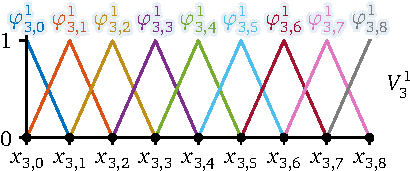
\includegraphics{hierarchicalBasis_1}%
  }%
  \hfill%
  \subcaptionbox{%
    Piecewise linear interpolant $\fgintp{l}$
    of some function data $\objfun(\gp{l,i})$
    as a weighted sum of the nodal hat functions.%
  }[72mm]{%
    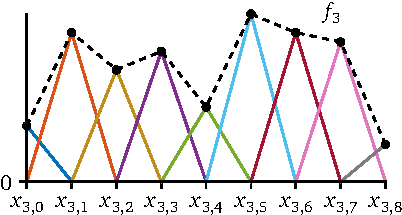
\includegraphics{interpolant_1}%
  }%
  \caption[%
    Univariate nodal hat functions%
  ]{%
    Univariate nodal hat functions of level $l = 3$.%
  }%
  \label{fig:nodalHat}%
\end{figure}



\subsection{Multivariate Case}
\label{sec:212nodalMV}

\paragraph{Cartesian and tensor products}

\usenotation{d}
For the multivariate case with $d \in \nat$ dimensions,
we employ a tensor product approach,
for which we replace all indices, points, and functions with
multi-indices, Cartesian products, and tensor products, respectively.
\usenotation{@0}
\usenotation{@1}
Therefore, the domain is now $\clint{\*0, \*1} \ceq \clint{0, 1}^d$,
which can be partitioned into
$\prod_{t=1}^d 2^{l_t} = 2^{\normone{\vec{l}}}$ equally-sized hyper-rectangles,
where $\*l = (l_1, \dotsc, l_d) \in \natz^d$ is the $d$-dimensional level
and $\normone{\vec{l}} \ceq \sum_{t=1}^d \abs{l_t}$ is the level sum.
The corners of the hyper-rectangles are given by the grid points
\begin{equation}
  \label{eq:gridPointMultivariate}
  \gp{\*l,\*i} \ceq \*i \cdot \ms{\*l},\quad
  \*i = \*0, \dotsc, \*2^{\*l}.
\end{equation}
Relations and operations with vectors in bold face
are to be read coordinate-wise in this thesis, unless stated otherwise.
Bold-faced numbers like $\*0$ are defined to be the vector $(0, \dotsc, 0)$
in which every entry is equal to that number.
This is to allow a somewhat intuitive and suggestive notation.
For example, \eqref{eq:gridPointMultivariate} is equivalent to
the much longer formula
\begin{equation}
  \gp{\*l,\*i}
  \ceq (i_1 \ms{l_1},\; \dotsc,\; i_d \ms{l_d}),\quad
  i_t = 0, \dotsc, 2^{l_t},\quad
  t = 1, \dotsc, d,
\end{equation}
with the $d$-dimensional mesh size
$\ms{\*l} \ceq \*2^{-\*l} = (\ms{l_1}, \dotsc, \ms{l_d})$.
Again, every grid point is associated with a basis function that is defined
as the tensor product of the univariate functions:%
\footnote{%
  Note that,
  although \cref{eq:tensorProduct} does not cover it,
  one could employ basis functions of different types in
  each dimension, for example B-splines of different degrees.
  All remaining considerations in this thesis
  regarding tensor product basis functions are independent
  of whether we use the same function type or
  different types in each dimension.%
}
\begin{equation}
  \label{eq:tensorProduct}
  \basis{\*l,\*i}\colon \clint{\*0, \*1} \to \real,\quad
  \basis{\*l,\*i}(\*x)
  \ceq \prod_{t=1}^d \basis{l_t,i_t}(x_t).
\end{equation}
\cref{fig:nodalHat2D} shows an example of a bivariate nodal hat function
$\bspl{\*l,\*i}{1}$.

\begin{SCfigure}
  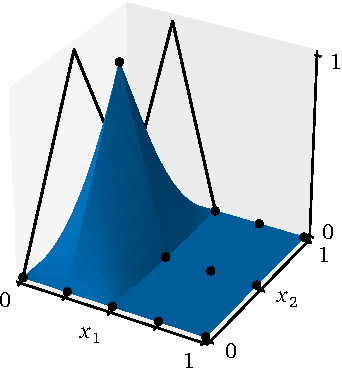
\includegraphics{nodalHat2D_1}%
  \caption[%
    Bivariate nodal hat function%
  ]{%
    Bivariate nodal hat function of level $\*l = (2, 1)$ and
    index $i = (1, 1)$ as the tensor product of two univariate
    nodal hat functions.%
  }%
  \label{fig:nodalHat2D}%
\end{SCfigure}

\vspace*{\fill}
\pagebreak

\paragraph{Multivariate nodal space}

The multivariate nodal space $\ns{\*l}$ is defined analogously to
the univariate case:
\begin{equation}
  \ns{\*l}
  \ceq \spn\{\basis{\*l,\*i} \mid \*i = \*0, \dotsc, \*2^{\*l}\}.
\end{equation}
In the case of hat functions $\bspl{\*l,\*i}{1}$,
the nodal space $\nsbspl{\*l}{1}$ is the $d$-linear spline space
\cite{Hoellig13Approximation}, i.e.,
the space of all continuous functions
on $\clint{\*0, \*1}$ that are piecewise $d$-linear polynomials on
all hyper-rectangles
\begin{equation}
  \clint{\gp{\*l,\*i}, \gp{\*l,\*i+\*1}}
  \ceq \clint{\gp{l_1,i_1}, \gp{l_1,i_1+1}} \times \dotsb \times
  \clint{\gp{l_d,i_d}, \gp{l_d,i_d+1}},\quad
  \*i = \*0, \dotsc, \*2^\*l - \*1.
\end{equation}
Analogously to \eqref{eq:interpFullGridUV},
we can interpolate objective functions $\objfun\colon \clint{\*0, \*1} \to \real$
in the nodal space $\ns{\*l}$ with $\fgintp{\*l}\colon \clint{\*0, \*1} \to \real$ satisfying
\begin{equation}
  \label{eq:interpFullGridMV}
  \fgintp{\*l}
  = \sum_{\*i=\*0}^{\*2^\*l} \interpcoeff{\*l,\*i} \basis{\*l,\*i},\quad
  \falarge{\*i = \*0, \dotsc, \*2^\*l}{\fgintp{\*l}(\gp{\*l,\*i}) = \objfun(\gp{\*l,\*i})},
\end{equation}
where $\interpcoeff{\*l,\*i} \in \real$ and
the sum is over all $\*i = \*0, \dotsc, \*2^\*l$
(i.e., $i_t = 0, \dotsc, 2^{l_t}$, $t = 1, \dotsc, d$).
To ensure that the coefficients $\interpcoeff{\*l,\*i}$
exist for every objective function $\objfun$ and are uniquely determined by
the values at the grid points
\begin{equation}
\fgset{\*l}
\ceq \{\gp{\*l,\*i} \mid \*i = \*0, \dotsc, \*2^{\*l}\},
\end{equation}
we prove the following statement:

\vspace*{\fill}
\pagebreak

\begin{lemma}[linear independence of tensor products]
  \label{lemma:tensorProductLinearIndependence}
  The functions $\basis{\*l,\*i}$ ($\*i = \*0, \dotsc, \*2^\*l$)
  form a basis of $\ns{\*l}$, if the univariate functions
  $\basis{l_t,i_t}$ ($i_t = 0, \dotsc, 2^{l_t}$)
  form a basis of the univariate nodal space $\ns{l_t}$
  for $t = 1, \dotsc, d$.
\end{lemma}
\begin{proof}
  Assume that $\interpcoeff{\*l,\*i} \in \real$ are chosen in \eqref{eq:interpFullGridMV}
  such that $\fgintp{\*l} \equiv 0$.
  Then for all $\*i' = \*0, \dotsc, \*2^\*l$,
  we can evaluate \eqref{eq:interpFullGridMV} at $\gp{\*l,\*i'}$ to obtain
  \begin{equation}
    \sum_{i_1=0}^{2^{l_1}}
    \paren*{
      \sum_{i_2=0}^{2^{l_2}} \dotsb \paren*{
        \sum_{i_d=0}^{2^{l_d}}
        \interpcoeff{\*l,\*i} \basis{l_d,i_d}(\gp{l_d,i_d'})
      } \dotsb \basis{l_2,i_2}(\gp{l_2,i_2'})
    } \basis{l_1,i_1}(\gp{l_1,i_1'})
    = 0.
  \end{equation}
  We apply the univariate linear independence ($x_1$ direction) to infer
  that the sum over $i_2$ must vanish for all $i_1 = 0, \dotsc, 2^{l_1}$.
  Repeating this argument for all dimensions, we have
  $\interpcoeff{\*l,\*i} = 0$ for all~$\*i = \*0, \dotsc, \*2^\*l$,
  implying the linear independence of the functions $\basis{\*l,\*i}$.
\end{proof}

\usenotation{n10}
A common choice for the level $\*l$ is $n \cdot \*1$ for some $n \in \natz$.
\usenotation{Vnd}
In this case, we replace ``$\*l$'' in the subscripts with ``$n{,}d$''
(for example, $\ns{n,d} \ceq \ns{n \cdot \*1}$).
For the hat function basis $\bspl{\*l,\*i}{1}$,
it can be shown that the $\Ltwo$ interpolation error of the interpolant
$\fgintp{n,d} \in \ns{n,d}$ is given by
\begin{equation}
  \normLtwo{\objfun - \fgintp{n,d}} = \landauO{\ms{n}^2},
\end{equation}
i.e., the order of the interpolation error is quadratic in the mesh size
\multicite{Hoellig13Approximation,Bungartz04Sparse}.
